% LaTeX Template for short student reports.
% Citations should be in bibtex format and go in references.bib
\documentclass[a4paper, 11pt]{article}
\usepackage[top=3cm, bottom=3cm, left = 2cm, right = 2cm]{geometry} 
\geometry{a4paper} 
\usepackage[utf8]{inputenc}
\usepackage{textcomp}
\usepackage{graphicx} 
\usepackage{amsmath,amssymb}  
\usepackage{bm}  
\usepackage[pdftex,bookmarks,colorlinks,breaklinks]{hyperref}  
%\hypersetup{linkcolor=black,citecolor=black,filecolor=black,urlcolor=black} % black links, for printed output
\usepackage{memhfixc} 
\usepackage{pdfsync}  
\usepackage{fancyhdr}
\usepackage{tikz}
\pagestyle{fancy}

\title{\textbf{Sistema de Seguridad implementado en LabVIEW con comunicación de APIs}}
\author{Daniel Alejandro Martínez Lara}
%\date{}

\begin{document}
\maketitle

\begin{tikzpicture}[remember picture,overlay]
    %-----------LOGOS
    \node[anchor=center,scale=.3,xshift=9cm,yshift=-7cm] (uaslpl) at (current page.north west){
\includegraphics{images/LOGO_UASLP_AZUL.png}};

    \node[anchor=center,scale=.15,xshift=85cm,yshift=2cm] (iicologo) at (uaslpl.east){
\includegraphics{images/LOGO_IICO_AZUL.png}};

    %----------Imagen de fondo

    \node[anchor=center,scale=.31,xshift=0cm,yshift=0cm] (bg) at (current page.center){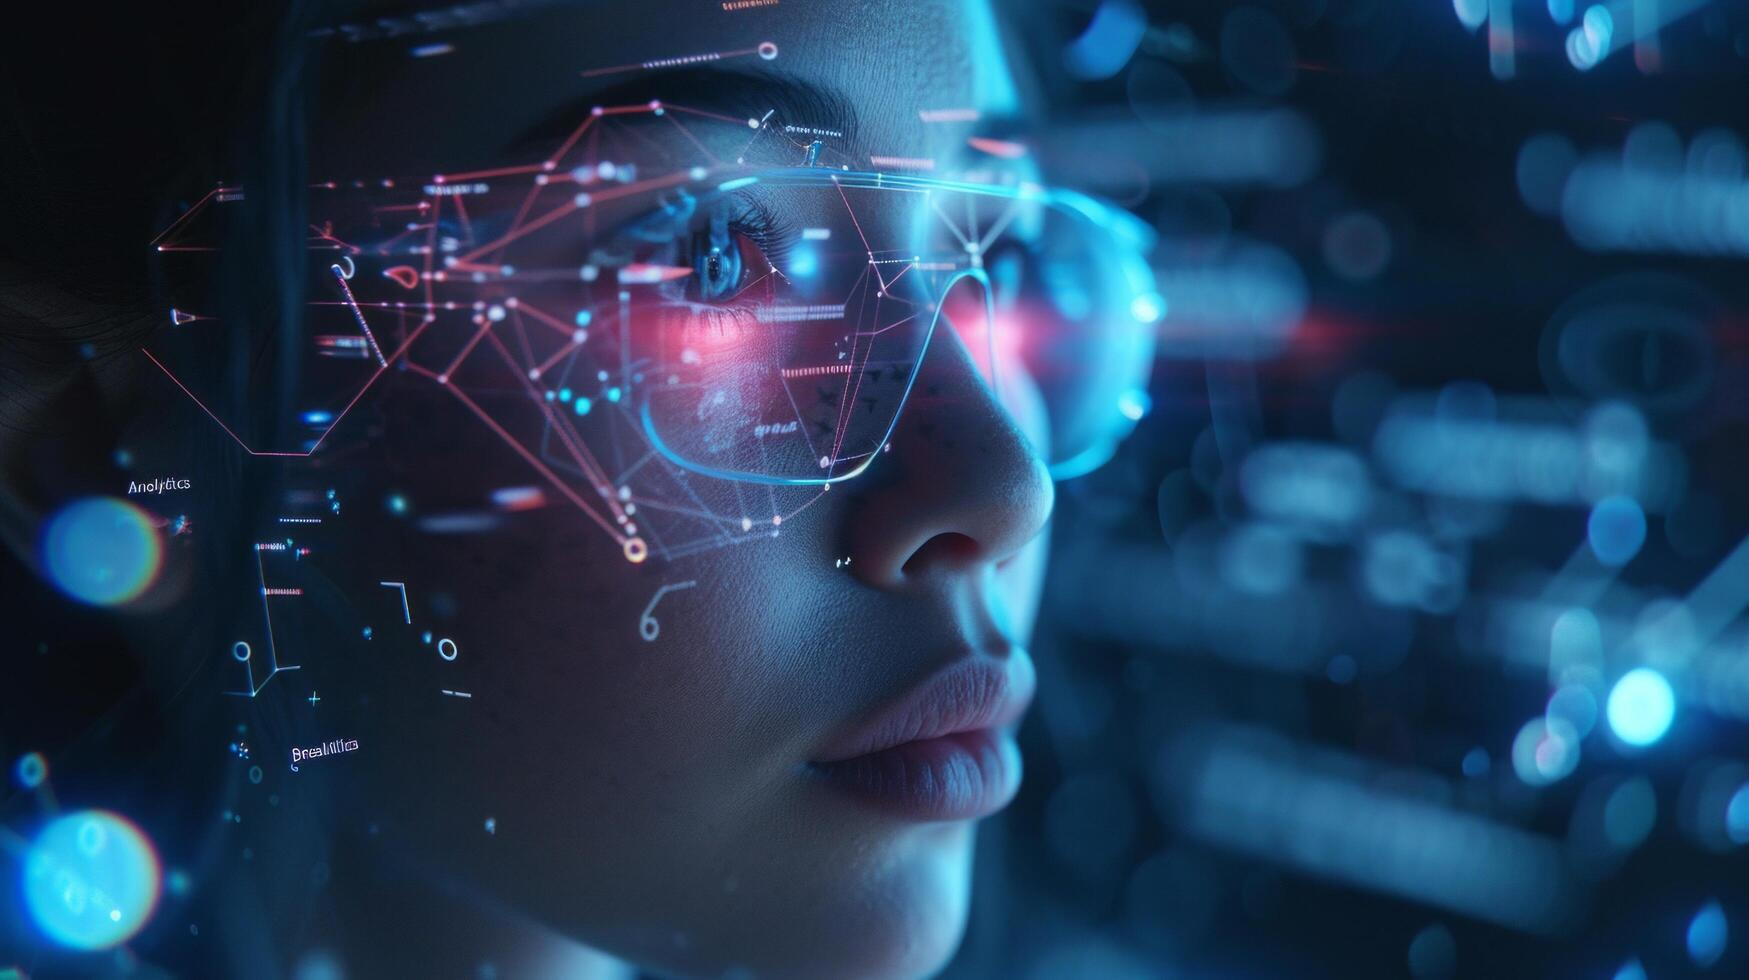
\includegraphics{images/recog-background.jpeg}};


    \node[anchor=center,scale=1,xshift=0cm,yshift=-8cm,text width=16cm,align=center] (txsouth) at (current page.center){
        \textbf{MATERIA:} LABORATORIO DE INSTRUMENTACIÓN VIRTUAL\\
        \textbf{DOCENTE:} MEJÍA CARLOS MARCELA, L.S.C.
    };

\end{tikzpicture}

\newpage
\tableofcontents

\section{Introducción}

Durante el desarrollo de la materia de LabVIEW se tocó el tema acerca de la implementación de APIs en el programa, facilitando procesos de reconocimiento de imágenes ya que primeramente empezamos con el sistema VISION integrado en LabVIEW, pero con la limitación de lo impreciso que podía ser el programa.\\
Con esta migración a un nuevo sistema de reconocimiento es que comenzó un interés por estos sistemas.
Ya que esta aplicación trata del trabajo en la curiosidad de cómo podía implementarse a un sistema de
seguridad.

\begin{tikzpicture}[remember picture,overlay]
    \node[anchor=center,scale=.15,xshift=-30cm,yshift=-50cm] at (current page.center){
\includegraphics{images/labviewlogo.jpeg}};

    \node[anchor=center,scale=.04,xshift=0cm,yshift=-120cm] at (current page.center){
\includegraphics{images/Amazon-Web-Services-AWS-Logo.png}};

    \node[anchor=center,scale=.5,xshift=10cm,yshift=-15.5cm] at (current page.center){
\includegraphics{images/Google-Cloud-Logo-PNG-Pic.png}};
\end{tikzpicture}

\pagebreak

\section{Objetivos}

Para este proyecto tenemos los siguientes objetivos a cumplir durante el desarrollo del programa:
\begin{itemize}
    \item Implementación de escaneo de código QR para el programa.
    \item Verificación de existencia del usuario dentro de una base de datos basada en Google Sheets.
    \item Verificación de equipo de seguridad del usuario para autorizar su acceso.
    \item Registro de cada intento de acceso y cada acceso autorizado por parte de los usuarios.
\end{itemize}

\section{Programa Principal}

Esta sección se separó en distintas etapas donde se explica en profundidad cada función del programa y del porqué se tomaron las decisiones de usar librerías y funciones dentro de LabVIEW y Python.
\\
\\
\textbf{Principalmente se implementó el uso de Python para librerías como gspread para la conexión sencilla entre tokens y usuario ya que en LabVIEW se topaba con la dificultad de refrescar el token cada cierto tiempo, permitiendo así al usuario eliminar dicha preocupación y únicamente ocuparse del funcionamiento del programa.}

\pagebreak

\subsection{Programas de Python (Reconocimiento del Usuario)}

Como primera implementación se utilizó el siguiente código de Python.

\begin{figure}[ht]
    \centering
    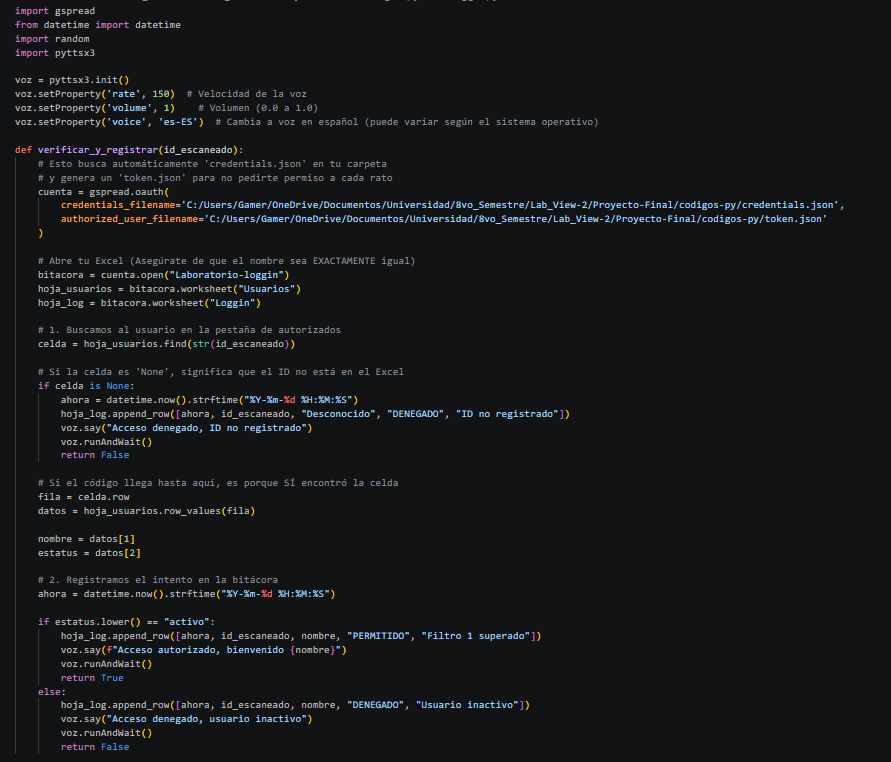
\includegraphics[scale=.7]{images/logincode1.png}
    \caption{Código de acceso al usuario.}
\end{figure}

Este código se encarga de recibir como entrada un valor numérico, para después acceder a las credenciales del usuario para poder inicializar los servicios de Google.
\\
Una vez con esto entra dentro de Google Spreadsheets para acceder a la base de datos del sistema, guarda una variable para acceder a la bitácora de accesos y otra variable para la hoja de usuarios dentro del sistema.
\\
\\
En este caso estamos buscando a un usuario por lo que leemos la hoja para encontrar el id escaneado, en caso de que no lo encuentre nos manda un mensaje de error diciéndonos que el usuario no se encuentra dentro de la base de datos de usuarios registrados.
\\
En caso de encontrar al usuario guardamos el número de fila y columna y extraemos los datos de esa fila para darle la bienvenida al usuario, además de acceder a la hoja encargada de la bitácora para poder guardar el acceso al PRIMER filtro.

\pagebreak
\subsection{Programas de Python (Reconocimiento de equipo)}

Como segunda implementación se utilizó el siguiente código.
\begin{figure}[ht]
    \centering
    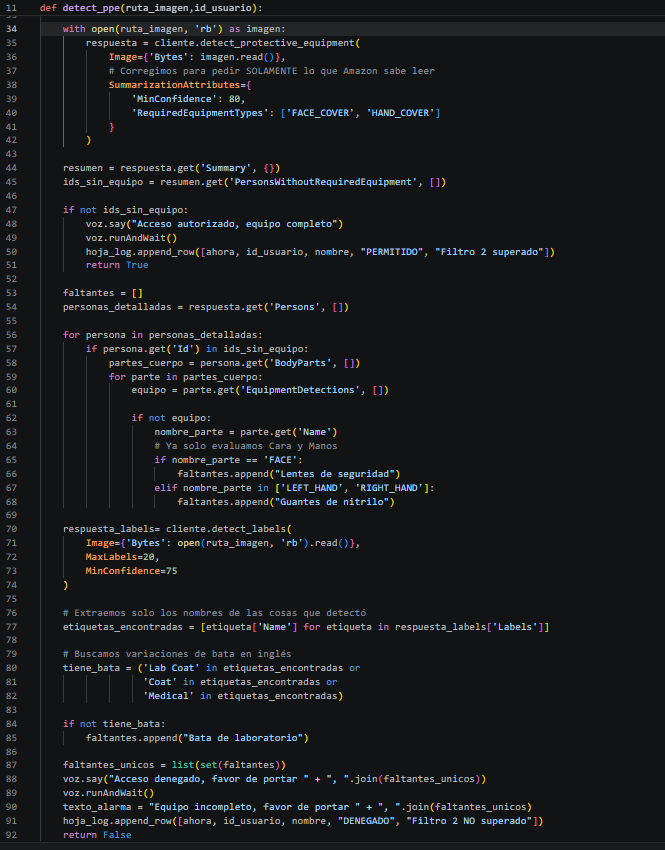
\includegraphics[scale=.7]{images/logincode2.png}
    \caption{Código de Verificación de equipo.}
\end{figure}

Para este caso el código se encarga de recibir la imagen a la cual le va a aplicar reconocimiento, el id\_usuario se recibe para un sistema de voz implementado por medio de la librería \textbf{pyttsx3}. Con la imagen obtenida el programa la abre y define los atributos con los cuales va a ser el score mínimo para detectar el objeto, en este caso checaremos que el usuario lleve cubierta la cara con lentes de seguridad y guantes para laboratorio.\\
Guardamos los resultados del escaneo que realiza la API y en caso de que la variable "ids\_sin\_equipo" esté vacía significa que el usuario cuenta con los equipos necesarios para entrar al laboratorio y realizamos un escaneo adicional para verificar que la persona cuente con una bata de seguridad.
Cuando se cuenta con el equipo completo el sistema nos dará acceso, en caso contrario el sistema nos comentará del equipo que hace falta portar.

\pagebreak

\subsection{Interfaz de LabVIEW (Conexión con Python)}
La conexión con LabVIEW se realizó de la siguiente forma.
\begin{figure}[ht]
    \centering
    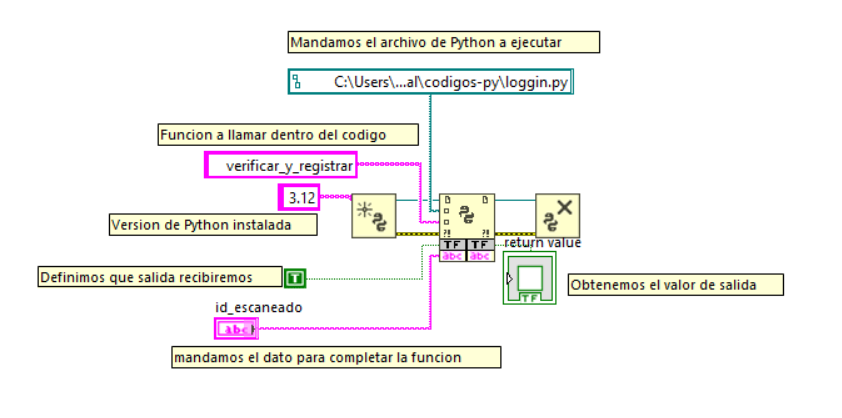
\includegraphics[scale=1]{images/lb-con1.png}
    \caption{Función de Python Node.}
\end{figure}
La función conocida como "Python Node" es una función que permite la interacción entre LabVIEW y Python en la cual inicializamos la sesión de Python donde definimos la versión de Python que utilizaremos para después mandar a llamar el archivo que ejecutaremos, a su vez le decimos qué función de nuestro programa desea que utilicemos y finalmente le definimos el tipo de salida que nos regresará el programa y el indicador de entrada que recibirá el código.

\subsection{Programa en LabVIEW pt.1}
El programa de LabVIEW nos recibe con la siguiente comparación de booleanos para verificar a qué estado nos mandará, ya que este programa está regido por una máquina de estados.

\begin{figure}[ht]
    \centering
    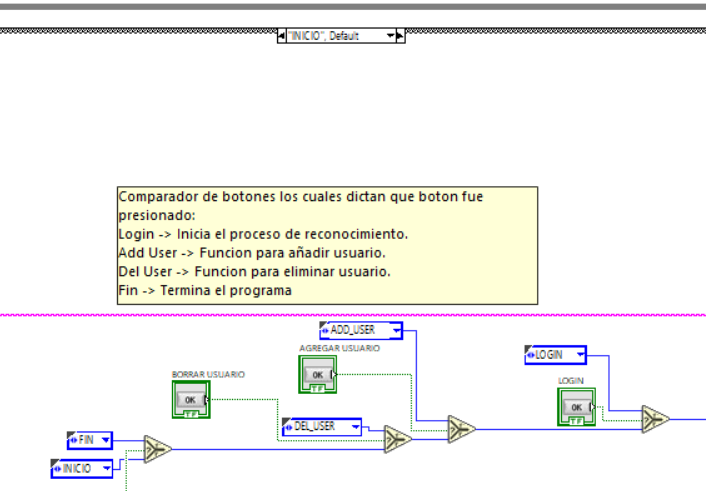
\includegraphics[scale=.5]{images/lb-con2.png}
    \caption{Estado de "INICIO" del programa.}
\end{figure}

Cuando escogemos el botón de "Search" iniciamos el proceso de login, donde el programa realiza la siguiente función.

\begin{figure}[ht]
    \centering
    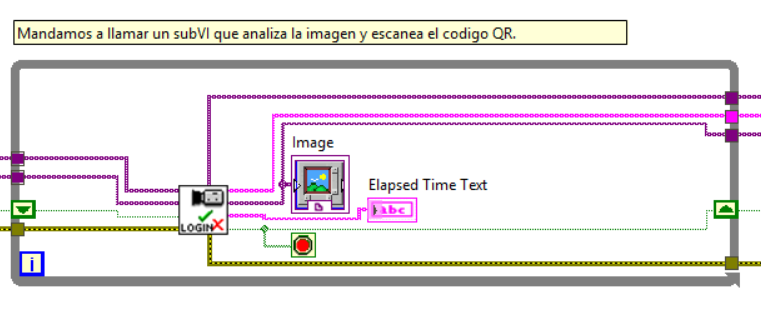
\includegraphics[scale=.7]{images/lb-con3.png}
    \caption{Utilización de subVI especializado.}
\end{figure}

El programa recibe la imagen actual del programa para entrar a un subVI que se encarga de analizar el código QR que el usuario tiene.

\begin{figure}[ht]
    \centering
    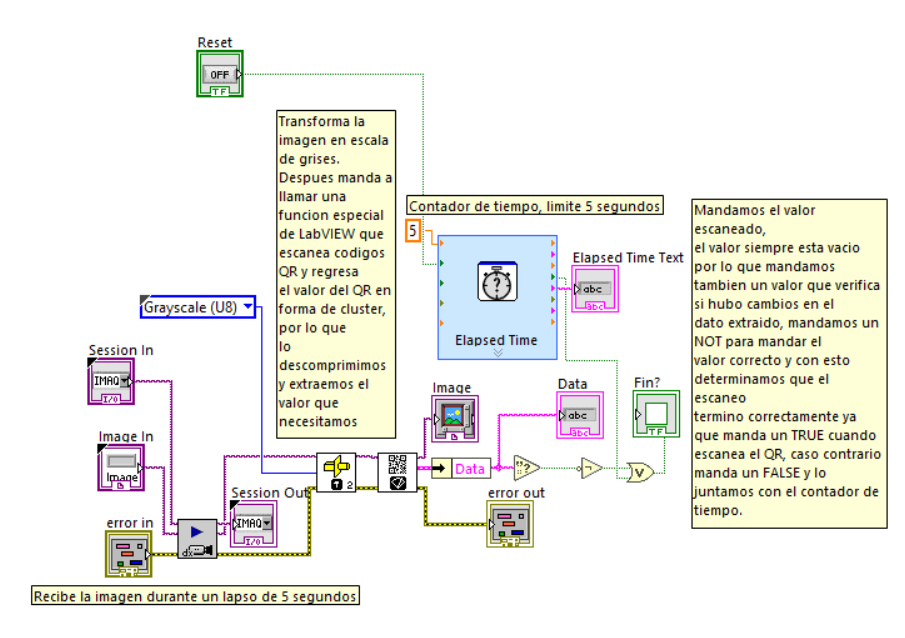
\includegraphics[scale=.7]{images/lb-con4.png}
    \caption{Escaneo de QR.}
\end{figure}

Este subVI recibe la imagen continuamente durante 5 segundos como límite, en caso de superar esos 5 segundos el escaneo termina y regresa un valor vacío.
En caso de que encuentre un código QR capaz de escanear lo escanea y regresa en forma de cluster el valor que encuentra dentro del QR, por lo que descomprimimos lo que regresa la función integrada a LabVIEW y sacamos únicamente el valor escaneado, cuando este valor cambia está conectado a una función que está continuamente checando cuando cambia el valor de "Data" en caso de cambiar manda un booleano y lo invertimos con un NOT para evitar errores.

\subsection{Programa en LabVIEW pt.2}
Una vez que se obtiene algún ID o incluso puede mandar un número vacío (El cual Python tomará como 0), se manda a llamar el programa que realiza un barrido para buscar la ID del usuario y manda una respuesta.
\\
En caso de encontrar un usuario nos dará acceso a la segunda fase para realizar login, caso contrario nos regresará al inicio y nos dirá que el usuario no se encontró, TODO movimiento que hagamos se guardará en la bitácora de accesos ya sean accesos autorizados o denegados.
\begin{figure}[ht]
    \centering
    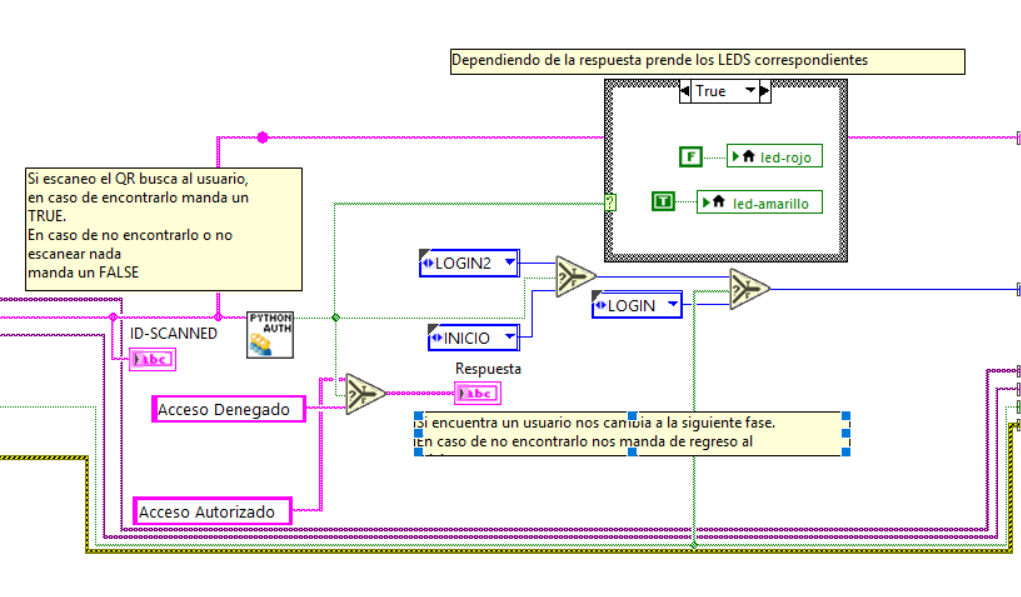
\includegraphics[scale=.7]{images/lb-con5.png}
    \caption{Escaneo de ID.}
\end{figure}

\pagebreak
\subsection{Programa en LabVIEW pt.3}
Cuando el usuario puede entrar a la fase 2 del sistema de logueo, se le da indicaciones que se quede de forma visible frente a la cámara ya que se le tomará una foto de ese momento preciso en el que acabe el mensaje dado por un script de Python.
\begin{figure}[ht]
    \centering
    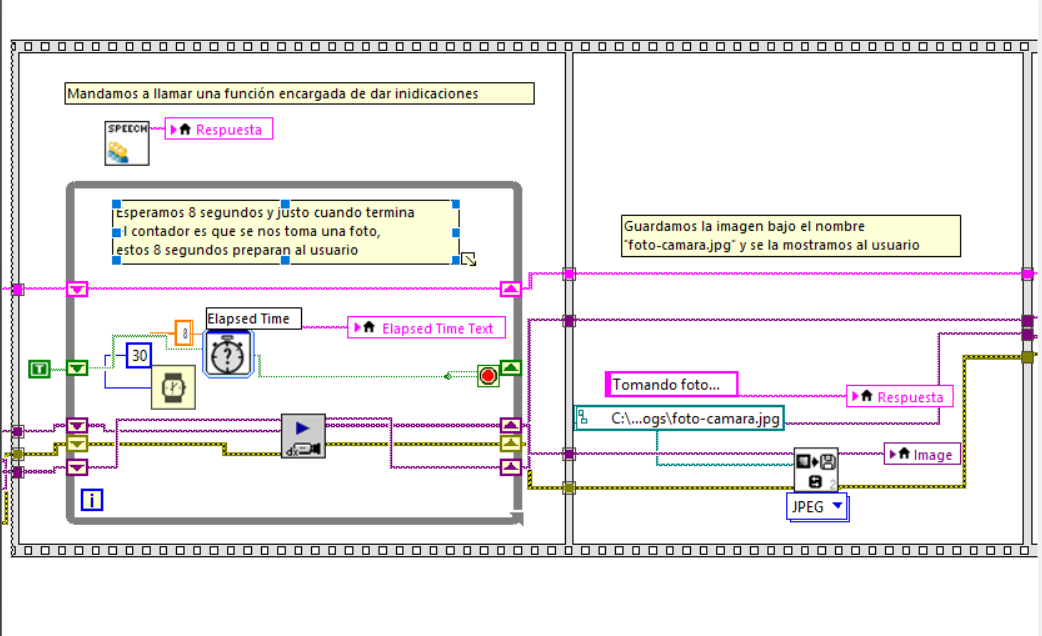
\includegraphics[scale=.5]{images/lb-con6.png}
    \caption{Login fase 2 pt1.}
\end{figure}

El sistema entra en un conteo de 8 segundos en los cuales la persona se tiene que preparar, una vez pasado ese tiempo se le tomará una foto.
\\
Dicha foto se guardará en forma de archivo con nombre "foto-camara.jpg" la cual se le mostrará al usuario.
\begin{figure}[ht]
    \centering
    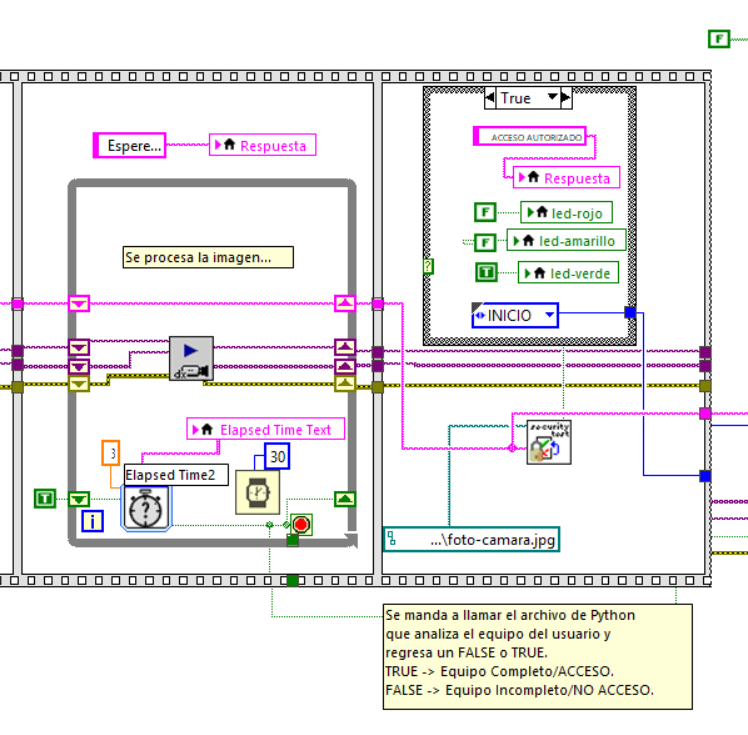
\includegraphics[scale=.5]{images/lb-con7.png}
    \caption{Login fase 2 pt2.}
\end{figure}

La foto será procesada, además de esperar 3 segundos para no saturar las tareas del sistema, después de ese tiempo se manda a llamar el script que explicamos anteriormente el cual analizará la imagen y nos entregará si el usuario cuenta con el equipo completo o hace falta que porte un equipamiento extra.
\section{Funciones Adicionales}
Como funciones adicionales se agregaron 2 para gestionar a los usuarios dentro del laboratorio dando esa libertad de eliminar o agregar usuarios a la base de datos encargada de monitorear a los usuarios que pueden entrar al laboratorio.
\subsection{Agregar Usuario}

La siguiente función es llamada por medio de Python ya que nuevamente es más fácil utilizar los servicios de Google, por lo que explicaremos el script.

\begin{figure}[ht]
    \centering
    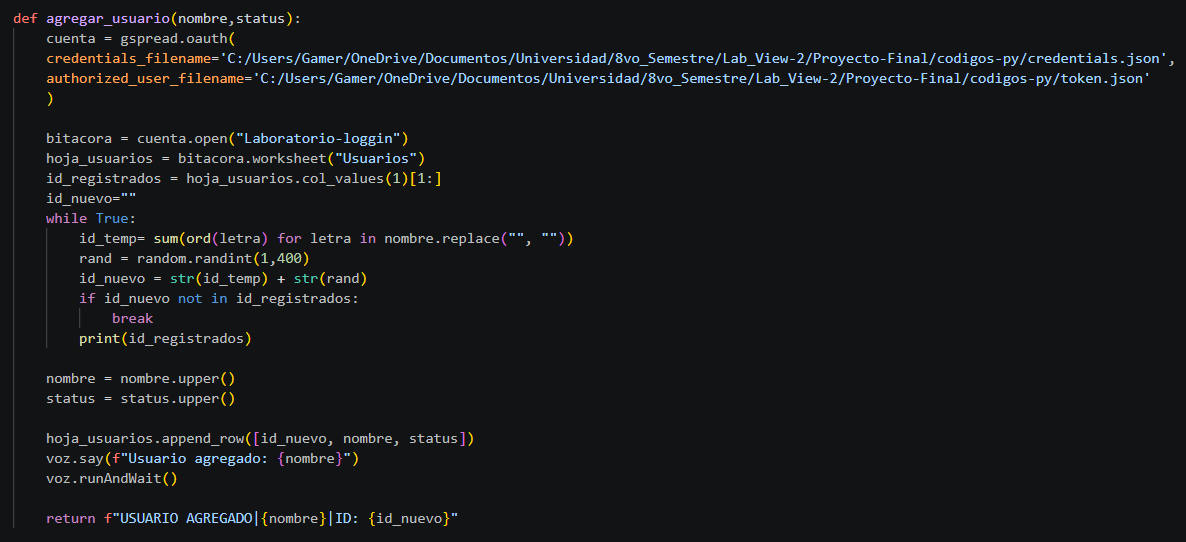
\includegraphics[scale=.5]{images/addcode1.png}
    \caption{Login fase 2 pt2.}
\end{figure}

Este script nuevamente accede a la base de datos pero dentro de su función recibe el nombre del usuario y manda automáticamente un estatus "activo", con el nombre de la persona y se va a la fila que esté vacía para poder agregar los datos de la persona, además de generar un ID basado en código ASCII de cada letra del nombre del usuario y después agregarle un número aleatorio, después verifica que la ID no esté registrada en el sistema, en caso de ya estar registrada sumamos un valor aleatorio hasta que encontremos un ID no utilizado y lo registra en la base de datos.
\pagebreak
\subsection{Eliminar Usuario}

La siguiente función es llamada por medio de Python ya que nuevamente es más fácil utilizar los servicios de Google, por lo que explicaremos el script.

\begin{figure}[ht]
    \centering
    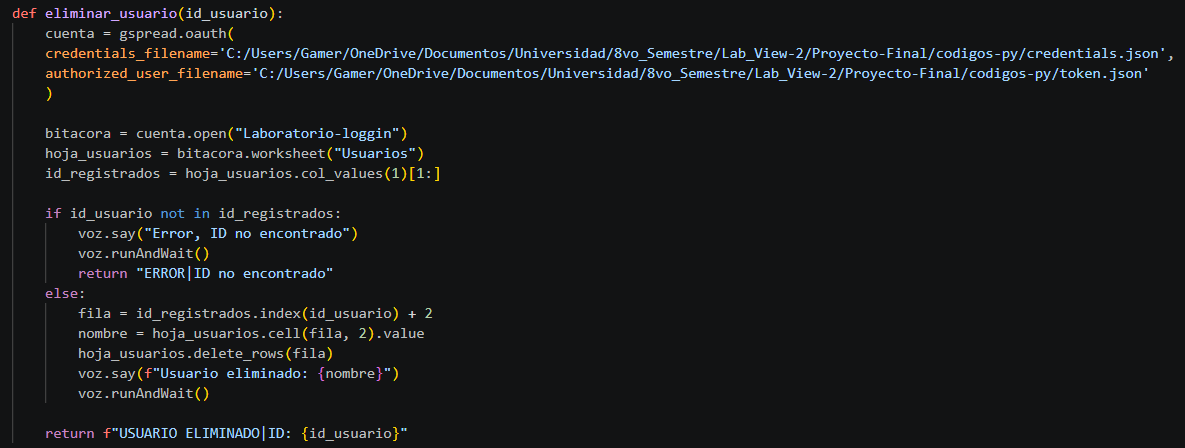
\includegraphics[scale=.5]{images/delcode1.png}
    \caption{Login fase 2 pt2.}
\end{figure}

Este script recibe únicamente la ID del usuario que se desea eliminar, posteriormente ingresa a la base de datos que mantiene a los usuarios activos y realiza un barrido el cual busca la ID del usuario, en caso de encontrarlo simplemente lo elimina, pero caso contrario nos menciona que la ID no se encontró.

\section{Panel Frontal [Resultado]}

Como resultado, se acomodó de la siguiente forma el panel frontal para permitir una interacción cómoda con el programa.

\begin{figure}[ht]
    \centering
    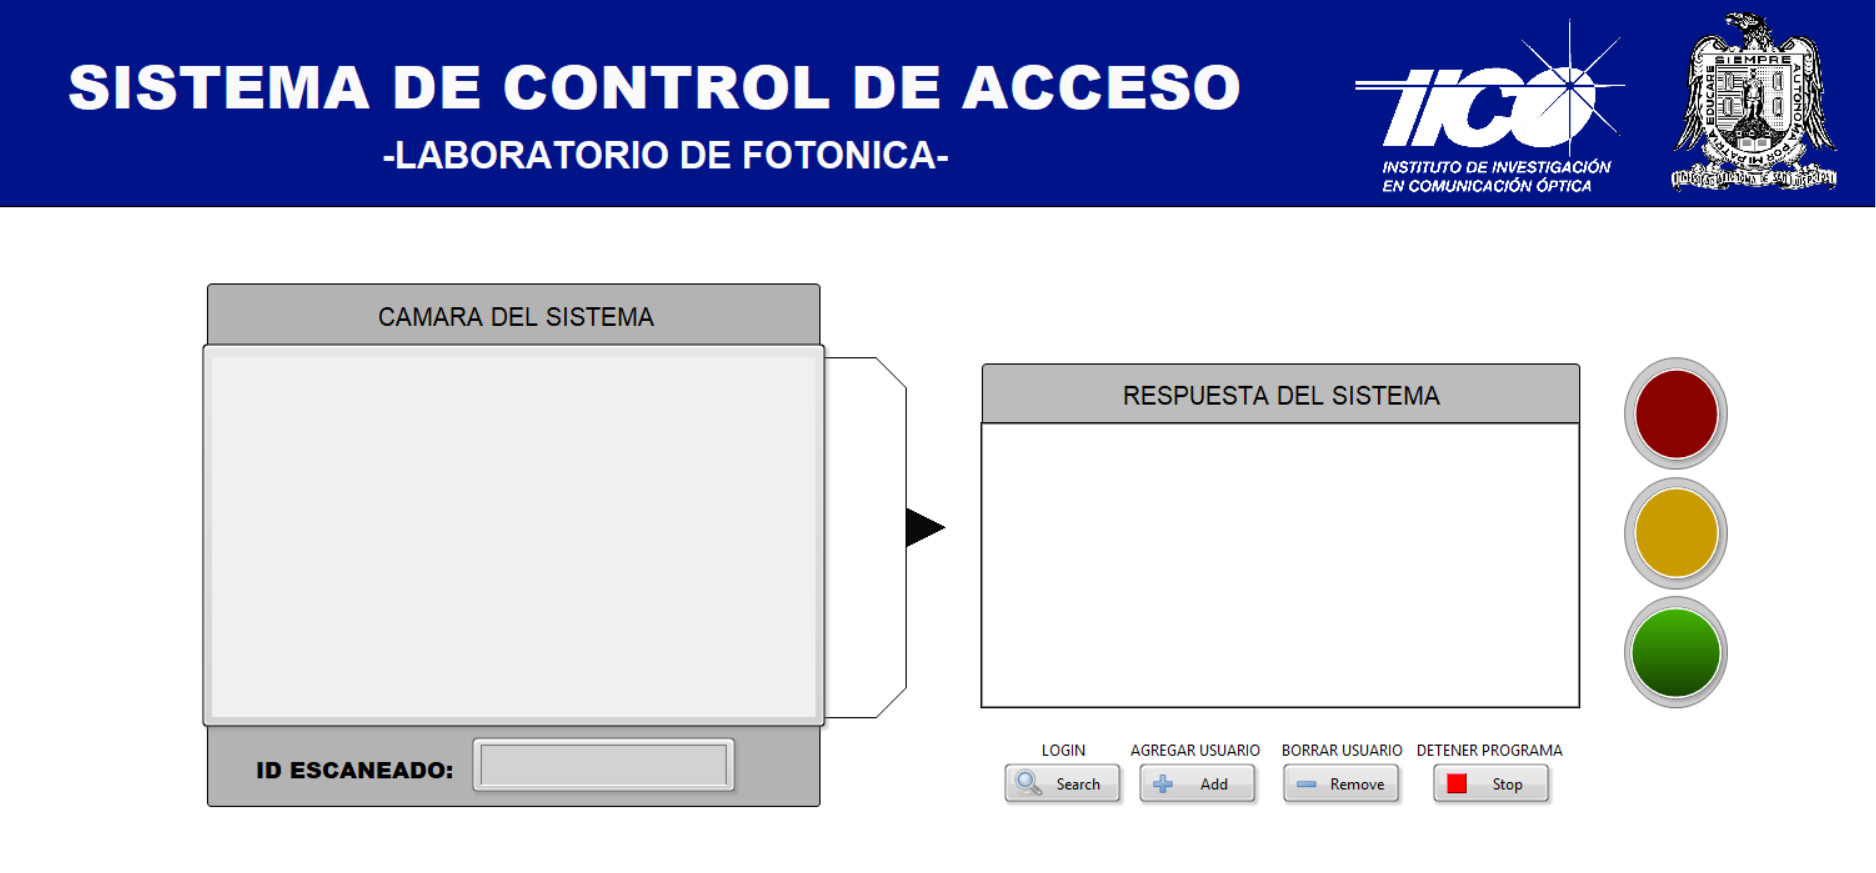
\includegraphics[scale=.3]{images/lb-con10.png}
    \caption{Panel Frontal.}
\end{figure}


\section{Conclusiones}

La elaboración de este proyecto permitió al usuario entender la interacción e implementación de APIs en Python y posteriormente su conexión con LabVIEW para así crear un programa interactivo que cumpla los objetivos esperados y propuestos para este proyecto.

\bibliographystyle{abbrv}
% \bibliography{references}  % need to put bibtex references in references.bib 
\end{document}